\chapter{Experimentos e Resultados}
\label{cap:experimentos-resultados}
%Este capítulo visa apresentar os testes executados durante o estudo e elaboração deste documento, assim como os resultados alcançados durante a construção. Abordar os principais pilares para a execução do desenvolvimento e verificação de validação dos testes para alcançar os objetivos do projeto. O desenvolvimento visou trabalhar a partir um escopo menor e ampliar posteriormente.

Três classificadores foram analisados para a identificação facial, sendo elas o Haar Cascade, histogramas e redes neurais convolucionais. As três opções são amplamente utilizadas para na área de reconhecimento facial. Neste caso, foi optado por utilizar o classificador Haar Cascade pela facilidade de utilização e de identificação de diferentes características que planejou-se eliminar durante a manipulação das imagens, com pouca necessidade de codificação. Neste caso, não foi considerado relevante o tempo de processamento das imagens e não foi avaliado os resultados de precisão que os modelos obtivessem. 

Para os experimentos de tratamento de imagem foram utilizados imagens diferentes disponibilizadas na internet escolhidas para compreender cenários diversos. Esses experimentos tinham como intuito verificar enquadramento e exclusão de regiões sem presença de pele humana em situações não controladas a fim de entender o comportamento a serem tratados. Os cenários escolhidos tratavam-se de imagens onde havia apenas uma pessoa por foto, onde a pessoa fotografada constava com o rosto angulado, com cabelo na frente do rosto e o fundo da foto com cores próximas a tons de pele, sem controle de iluminação. 

Com essas imagens foram executados testes de dimensionamento para identificação de rosto utilizando Haar Cascade. Por utilizar o Haar Cascade com treinamento para localização de rostos frontais, os testes resultaram apontaram para o uso de imagens com o rosto em posição frontal e com menor angulação possível. Também percebeu-se que o cabelo frente ao rosto não era excluído completamente durante o processamento da imagem, além da sombra que o cabelo causava influenciar no resultado de identificação de cores. Ademais, as cores de fundo das imagens não demonstraram influenciar nos resultados nos testes avaliados. Também percebeu-se que a identificação de tom de pele dominante nas imagens eram influenciados pelas regiões da face como o nariz, olhos, sobrancelha e boca, pela presença de sombreamento e a presença de pelos. 

A partir disso, baseado nos resultados dos testes do classificador, escolheu-se recortar as imagens onde o algoritmo identificou a face para minimizar influência de cabelo e de objetos. Após o foco na face, retirou-se a região dos olhos na imagem e verificou-se novamente os resultados da paleta dominante. Realizou-se o mesmo para a região do nariz e boca como pode ser visto na Figura \ref{fig: Etapas_de_teste_roi}.

As áreas excluídas são identificadas com Haar Cascade, cada área com seu modelo próprio de identificação, e pintadas de preto para retirada dos pixels. A retirada das áreas melhorou a percepção de coloração dominante na paleta resultante e aumentou a presença de cores mais próximas à paleta de Monk.

Com base no estudo \cite{Automatic_Skin_Tone_Extraction_for_Visagism_Applications} e a Tabela \ref{table:Tabela_comparativa_sistemas_de_cores} optou-se por utilizar um sistema de cor com bom desempenho individual. Como o sistema de cor HSV e YCrCb obtiveram resultados semelhantes, foi avaliado o comportamento de ambos sistemas nas fotos utilizadas anteriormente. O teste constituía em avaliar as imagens e verificar a distinção do uso do modelo HSV e YCrCb na identificação de pixel relevantes. Os testes obtiveram resultados semelhantes, como esperado, contudo o modelo HSV comparado ao modelo YCrCb trouxe mais definição de detalhes, o que pode ser verificado na Figura \ref{fig:x Etapas_de_teste_cores}.

\begin{figure}[h]
\centering
\caption{Comparação de resultados entre HSV e YCbCr. (1) Imagem de referência; (2) Imagem com HSV; e, (3) Imagem com YCbCr.}
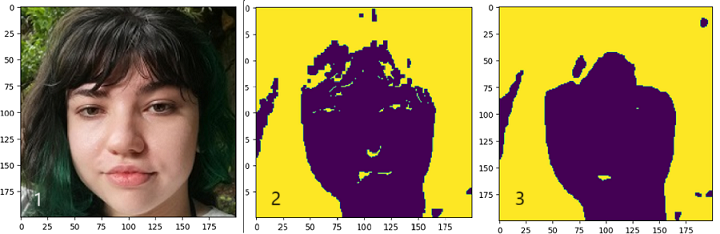
\includegraphics[scale=1.2]{Template_Latex_TCC-UNIFTEC/_lib/imagens/testHsvYcbcr.png}

\label{fig:x Etapas_de_teste_cores}
\centering{\Fonte{Autor}}
\end{figure}


Na Figura \ref{fig:x Etapas_de_teste_cores} a imagem (1) representa a imagem de referência, a (2) o resultado utilizando sistema de cor HSV e a imagem (3) o resultado utilizando o modelo YCbCr. Nota-se que no teste ambos sistemas distinguiram a região da face, contudo o modelo HSV retorna mais detalhes faciais comparado ao modelo YCbCr, o que pode auxiliar na identificação de pixels não relevantes na face, visto que o intuito é apenas o tom de pele.

Para a identificação dominante de tom de pele utilizando Kmeans avaliou-se alterar o parâmetro de n\_clusters. O parâmetro detém o valor de número de \textit{clusters},  assim como o número de centroides a ser utilizado. Em suma, o valor utilizado retorna a quantidade de cores identificadas por conjunto. Com isso, avaliou- se utilizar 1 a 10 , 15 e 20 \textit{clusters} nas imagens do \textit{dataset} MST-E para verificar qual configuração de \textit{clusters} retorna valores mais precisos. 

Com os testes com as 585 imagens do \textit{dataset} notou-se que a quantidade de \textit{cluster} não está relacionada a melhora na identificação da cor dominante. Utilizar menos \textit{clusters} na análise não trazem valores de cor dominantes mais próximas a cores da paleta de Monk, assim como utilizar mais \textit{clusters} não trazem melhores resultados. Além disso, para algumas imagens diferentes \textit{clusters} traziam os mesmos resultados de identificação. Contudo, nos testes utilizando 1, 2 e 3 \textit{clusters} algumas imagens não obtiveram resultado de cor dominante identificada sendo desconsiderados utilizar os \textit{clusters}. 

Além disso, para a validação de resultados de identificação de tom de pele dominante analisou-se duas formas diferentes para calcular a distância entre os tons da paleta de Monk e os tons dominantes encontrados. Na primeira avaliação, utilizou-se a distância euclidiana com o modelo RGB. Na segunda avaliação, utilizou-se a distância Delta E 2000 com o modelo CIELab que pode ser visto na Tabela \ref{table:Tabela_comparativa_entre_os_clusters_e_modelo_rgb} para o modelo RGB e a Tabela \ref{table:Tabela_comparativa_entre_os_clusters_e_modelo_cielab} para  modelo CIELab.

% \begin{table}[]
% \centering
% \caption{Tabela comparativa entre os clusters e modelos de cor}
% \label{table:Tabela_comparativa_entre_os_clusters_e_modelo}\textbf{}
% \resizebox{\columnwidth}{!}{%
% \begin{tabular}{lllllllll}
% \hline
% Clusters & RGB & \textgreater{}=1 & \textgreater{}=2 & \textgreater{}=3 & CIELab & \textgreater{}=1 & \textgreater{}=2 & \textgreater{}=3 &  \\ \hline
% 4        & 82  & 179              & 269              & 336              & 82     & 179              & 248              & 352              &  \\ 
% 5        & 68  & 180              & 270              & 329              & 75     & 174              & 259              & 347              &  \\ 
% 6        & 64  & 185              & 272              & 329              & 83     & 177              & 263              & 360              &  \\ 
% 7        & 67  & 182              & 265              & 330              & 80     & 173              & 256              & 352              &  \\ 
% 8        & 59  & 181              & 258              & 319              & 85     & 181              & 260              & 352              &  \\ 
% 9        & 65  & 171              & 262              & 322              & 82     & 181              & 263              & 342              &  \\ 
% 10       & 61  & 179              & 266              & 326              & 79     & 179              & 265              & 341              &  \\ 
% 15       & 69  & 180              & 269              & 328              & 84     & 187              & 266              & 349              &  \\ 
% 20       & 67  & 179              & 265              & 327              & 78     & 169              & 256              & 346              &  \\ \hline
% \end{tabular}%
% }
% \centering{\Fonte{Autor}}
% \end{table}

\begin{table}[h!]
\centering
\caption{Tabela comparativa entre os clusters e modelo RGB}
\label{table:Tabela_comparativa_entre_os_clusters_e_modelo_rgb}\textbf{}
\begin{tabular}{lllll}
\hline
Clusters & RGB & =1 &             =2 &             =3                \\ \hline
4        & 82  & 179              & 90               & 67            \\ 
5        & 68  & 180              & 90               & 59            \\ 
6        & 64  & 185              & 87               & 57            \\ 
7        & 67  & 182              & 83               & 65            \\ 
8        & 59  & 181              & 77               & 61            \\ 
9        & 65  & 171              & 91               & 60            \\ 
10       & 61  & 179              & 87               & 60            \\ 
15       & 69  & 180              & 89               & 59            \\ 
20       & 67  & 179              & 86               & 62            \\ \hline
\end{tabular}%
\centering{\Fonte{Autor}}
\end{table}%418

\begin{table}[h!]
\centering
\caption{Tabela comparativa entre os clusters e modelos CIELab}
\label{table:Tabela_comparativa_entre_os_clusters_e_modelo_cielab}\textbf{}
\begin{tabular}{lllll}
\hline
Clusters & CIELab & =1 &            =2 &                =3              \\ \hline
4        & 82     & 179              & 69               & 104           \\
5        & 75     & 174              & 85               & 88             \\ 
6        & 83     & 177              & 86               & 97             \\ 
7        & 80     & 173              & 86               & 96             \\ 
8        & 85     & 181              & 79               & 92             \\ 
9        & 82     & 181              & 82               & 79             \\ 
10       & 79     & 179              & 86               & 76             \\ 
15       & 84     & 187              & 79               & 83             \\ 
20       & 78     & 169              & 87               & 90             \\\hline
\end{tabular}%
\centering{\Fonte{Autor}}
\end{table} %437

Nos testes de validação de modelo das 595 imagens do \textit{dataset}, com o modelo RGB, conforme a Tabela \ref{table:Tabela_comparativa_entre_os_clusters_e_modelo_rgb} utilizar 4 \textit{clusters} retorna melhor desempenho para resultados iguais ao de Monk, contudo 4 \textit{clusters}, 82 imagens obtiveram os valores de classificação igual à classificação de Monk, enquanto 179 imagens tiveram diferença de um tom mais claro ou mais escuro na paleta de MonK, 90 imagens foram classificadas dois tons mais claros ou mais escuros do que a classificação de Monk e 67 imagens foram classificadas com 3 tons mais claros ou mais escuros. Os outros \textit{clusters} tiveram um desempenho significativamente menor considerando as classificações iguais.

Para o modelo CIELab, o melhor desempenho se demonstrou utilizando 8 \textit{clusters}. Sendo 85 imagens classificadas com o mesmo tom do que a classificação de Monk, 181 imagens classificadas com um tom mais claro ou mais escuro, 79 imagens classificadas dois tons mais claros ou mais escuro e 92 imagens classificadas com três tons mais claros ou mais escuros à classificação de Monk. 

Utilizar o modelo CIELab retornou resultados mais próximos à classificação de Monk no consistentemente entre os clusters comparado ao modelo RGB. Sendo o melhor resultado utilizar 8 \textit{clusters}. Sendo, 60,17\% das imagens com resultados próximos ao esperado. Por isso, decidiu-se utilizar o modelo CIELab para a validação de resultados e 8 \textit{clusters} na configuração do Kmeans.

Para fins de estudo e comparação de funcionamento, foi realizado testes de comparação entre paletas utilizando o sistema Casco e as imagens previamente selecionadas. Realizou-se uma comparação de resultados de cor dominante como pode ser visto na Figura \ref{fig:x PerlavsMonk} e por consequência a classificação de tom utilizando a paleta Monk e o programa desenvolvido com a paleta PERLA no artigo \cite{Classification_Algorithm_for_Skin_Color_CASCo_A_new_tool}

\begin{figure}[h]
\centering
\caption{Comparação de classificação paleta PERLA e Monk usando CASCo (1) Classificação PERLA; e, (2) Classificação Monk}
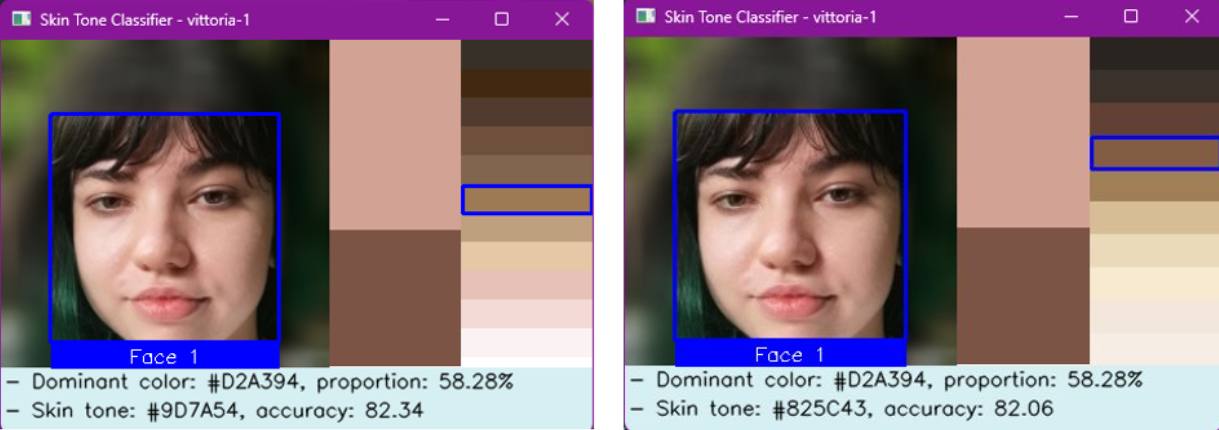
\includegraphics[scale=0.75]{Template_Latex_TCC-UNIFTEC/_lib/imagens/perlavsmonk.png}

\label{fig:x PerlavsMonk}
\centering{\Fonte{Autor}}
\end{figure}

Na Figura \ref{fig:x Etapas_de_teste_cores} a imagem (1) representa o teste utilizando o algoritmo CASCo com a paleta PERLA e a (2) representa o teste utilizando o algoritmo CASCo com a paleta de Monk. Os testes tinham intuito de entender o comportamento do algoritmo. O resultado comparativo destaca que na paleta de Monk o tom classificado ficou mais escuro comparado a paleta PERLA, apesar de ambas terem a mesma cor dominante selecionada. O que está relacionado a distribuições de tons entre as paletas. 